Once the local SimCenter working environment has been tested and is
functioning correctly, the \texttt{\getsoftwarename{}} Application
can be tested. The simplest way to do this is by running an analysis
using the default structural model with synthetic ground motions. By
doing this, it is not necessary to enter any information on the
structural model and only inputs for 
\softwareSwitch{PBE}{
the synthetic motions, uncertainty quantification, and loss assessment
}{
the synthetic motions and uncertainty quantification
}
are required. With this quick setup, the
functionality of the \texttt{\getsoftwarename{}} App and the backend
workflow can be tested. The necessary steps to perform this
testing are provided below.

A full description of how to use this software is provided
in \Cref{chap:usage}.  In this quick test, users will only
interface with the event tab (\texttt{EVT}), the uncertainty
quantification tab (\texttt{UQ}), 
\softwareSwitch{PBE}{
the damage and loss assessment tab (\texttt{CMP}),
}{}
and the results tab (\texttt{RES}).

The first step is to start the \texttt{\getsoftwarename{}}
application.  Once the application started, the second step is to
input the parameters for the synthetic motions under the \texttt{EVT}
(Event) tab. This is shown in \Cref{fig:input_event}. Click
on the \texttt{EVT} tab which will allow the loading type to be
selected. From the dropdown menu, as shown
in \Cref{fig:input_event}, select \texttt{Stochastic Ground Motion
Model}. Upon selecting this loading type, the loading model will be
set as \texttt{Vlachos et al. (2018)}.

\softwareSwitch{PBE}{
\begin{figure}[!htbp]
  \centering {
    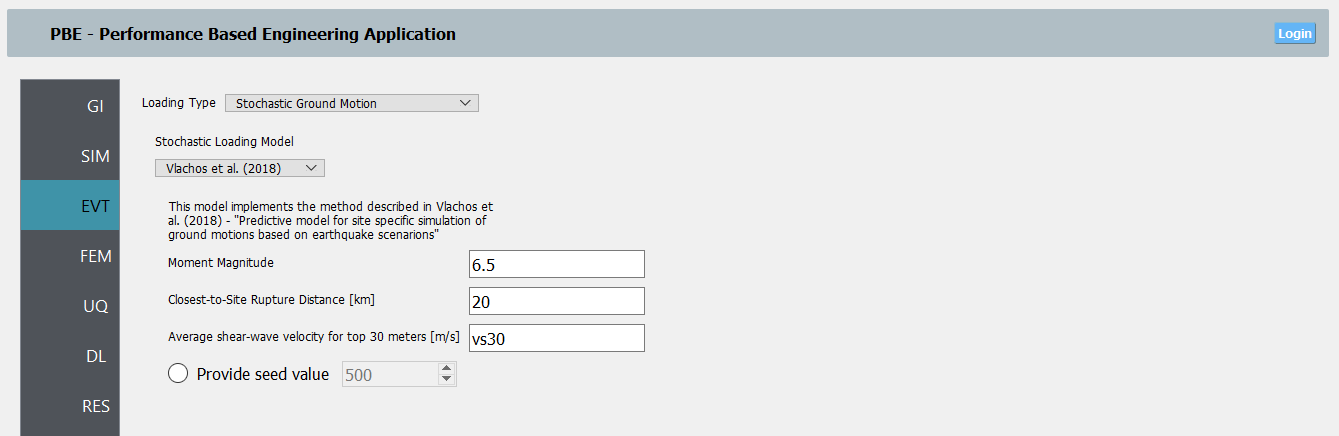
\includegraphics[width=0.95\textwidth]
    {installation/figures/test_input_event_pbe.png} }
  \caption{Selecting event type and inputting synthetic motion parameters}
  \label{fig:input_event}
\end{figure}
}{
\begin{figure}[!htbp]
  \centering {
    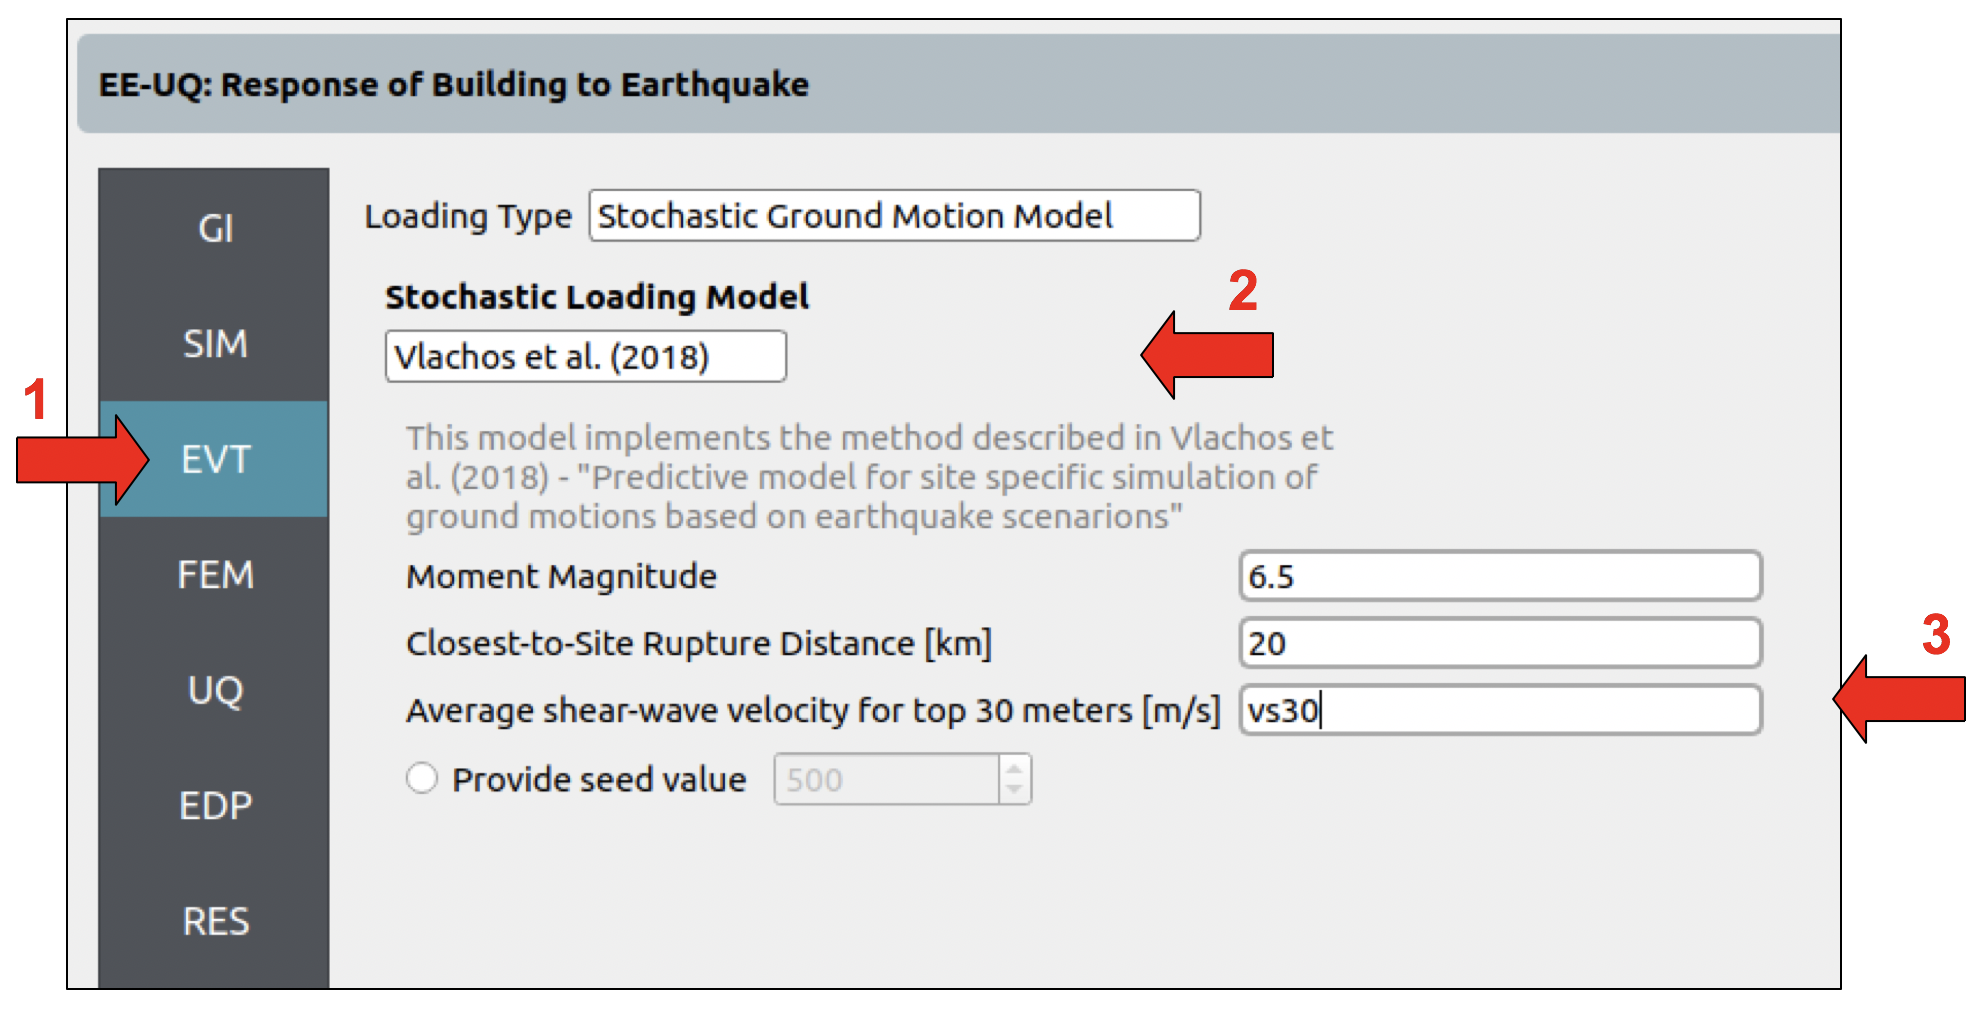
\includegraphics[width=0.7\textwidth]
    {installation/figures/test_input_event.png} }
  \caption{Selecting event type and inputting synthetic motion parameters}
  \label{fig:input_event}
\end{figure}
}

Only three inputs are required for this test, of which one will be set
to a random variable. As shown in \Cref{fig:input_event}, set the
\emph{Moment Magnitude} ($M_W$) to 6.5, the \emph{Closest-to-Site Rupture Distance}
($R_{rupt}$) to 20 km, and the \emph{Average shear-wave velocity
for the top 30 m} ($V_{S_{30}}$)
to \texttt{vs30}. The \texttt{Provide seed value} radio button should
be left unselected. By specifying these inputs, both $M_{W}$ and $R_{rupt}$
will have constant values in all realizations while $V_{S_{30}}$ will
have different values based on the model parameters specified in the
uncertainty quantification (\texttt{UQ}) tab.

With these inputs specified, navigate to the \texttt{UQ} tab. Here the
distributions and their relevant parameters will be specified for the
random variables defined in the analysis\textemdash only $V_{S_{30}}$
in this case. Since $V_{S_{30}}$ was identified as a random variable
by inputting the parameter value as text, it is automatically added as
a random variable, as shown in \Cref{fig:input_uq}. Set the
distribution type to \texttt{normal} with a \texttt{Mean}
and \texttt{Standard Dev} of 350 m/s and 25 m/s,
respectively.

\softwareSwitch{PBE}{
\begin{figure}[!htbp]
  \centering {
    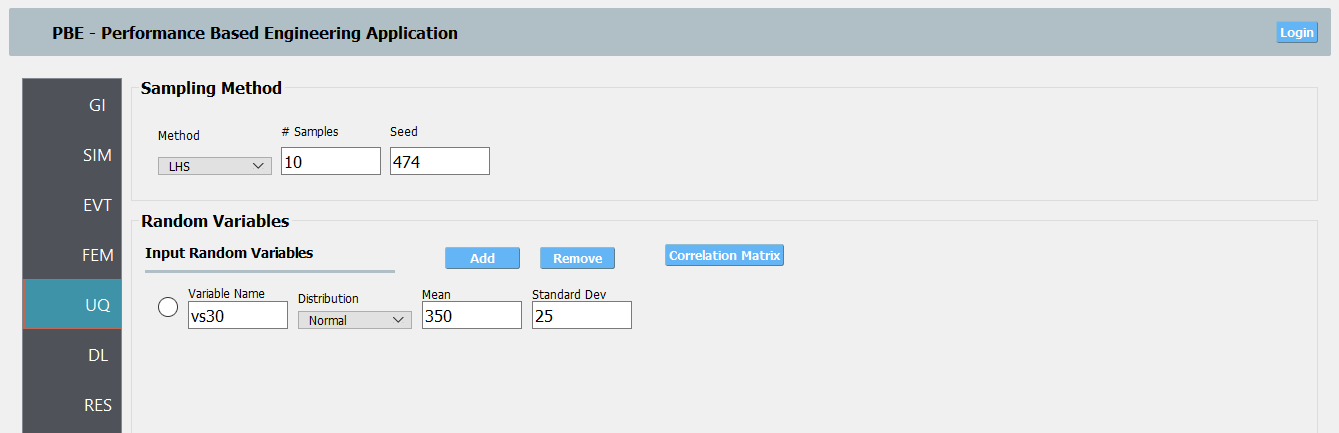
\includegraphics[width=0.95\textwidth]
    {installation/figures/test_input_uq_pbe.png} }
  \caption{Specifying distribution type and parameters for random
  variables in analysis\textemdash only $V_{s30}$ in this case}
  \label{fig:input_uq}
\end{figure}
}{
\begin{figure}[!htbp]
  \centering {
    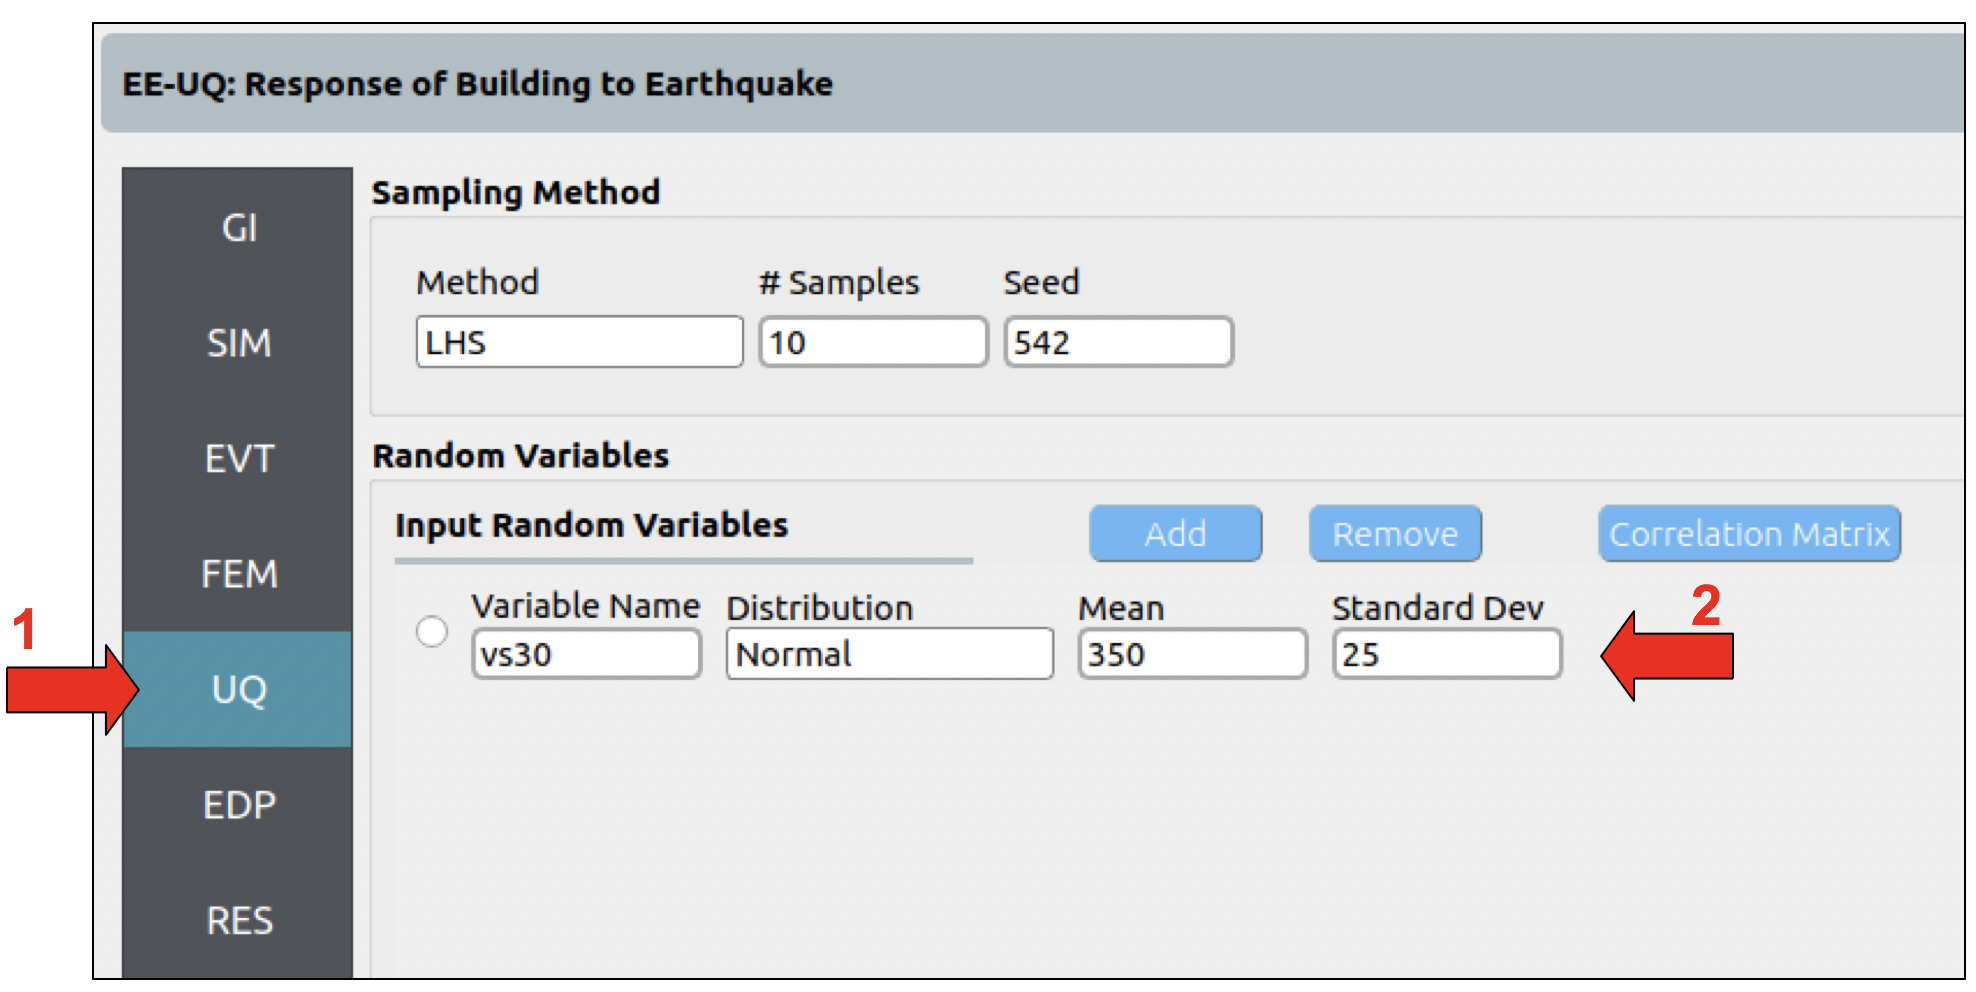
\includegraphics[width=0.7\textwidth]
    {installation/figures/test_input_uq.png} }
  \caption{Specifying distribution type and parameters for random
  variables in analysis\textemdash only $V_{s30}$ in this case}
  \label{fig:input_uq}
\end{figure}
}

\softwareSwitch{PBE}{
The last step before running the analysis is to set up a damage and loss model. Navigate to the \textttt{DL} tab and select \texttt{HAZUS MH} as the loss assessment method to use. Set up the model according to \Cref{fig:input_dl}.
\begin{figure}[!htbp]
  \centering {
    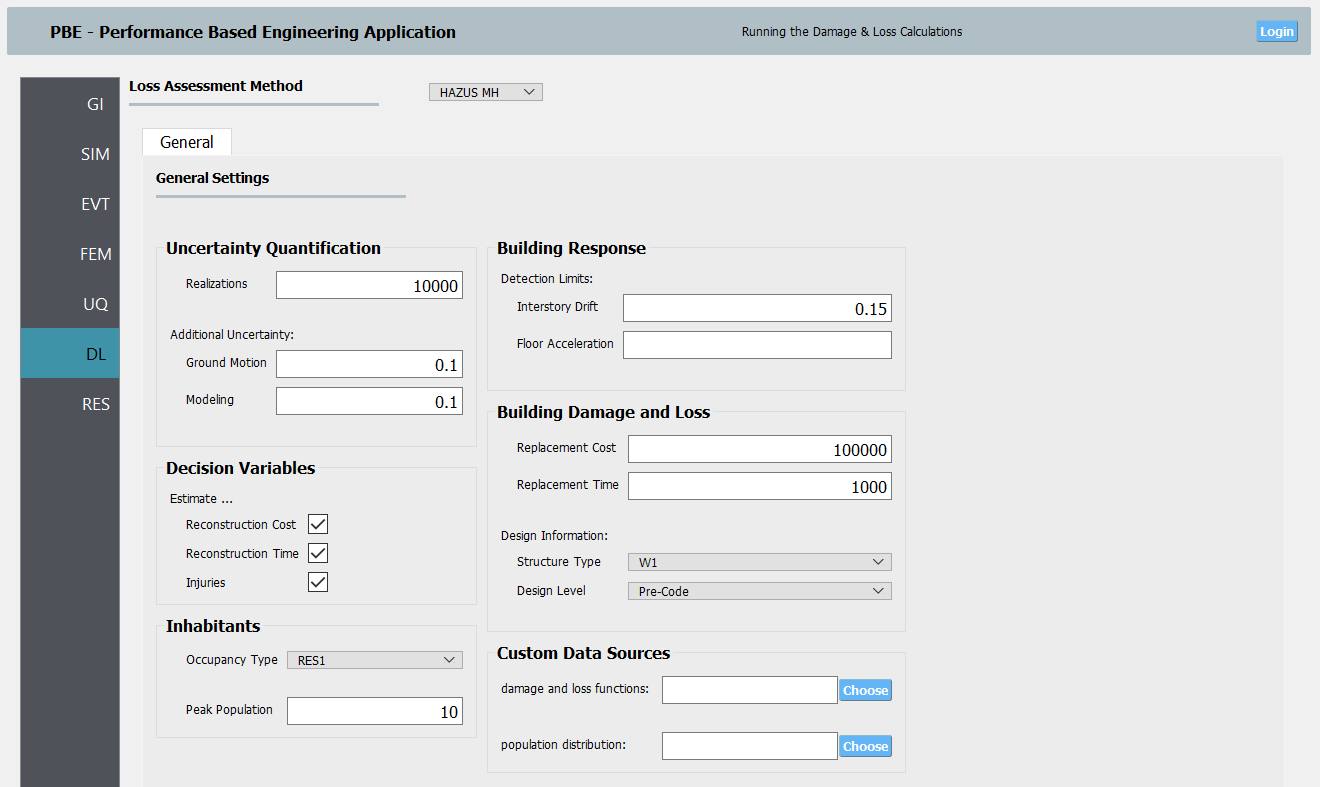
\includegraphics[width=0.95\textwidth]
    {installation/figures/test_input_dl.png} }
  \caption{Specifying the damage and loss model for the analysis.}
  \label{fig:input_dl}
\end{figure}
}{}

Now, click on the \texttt{RUN} button, which will bring up a pop-up
menu that provides information on the application directory and
the working directory. The application directory should already be
automatically set to where \texttt{\getsoftwarename{}} is installed.
If desired, the working directory can be changed. In order to start
the analysis, click on the \texttt{Submit} button.

\softwareSwitch{PBE}{
\begin{figure}[!htbp]
  \centering {
    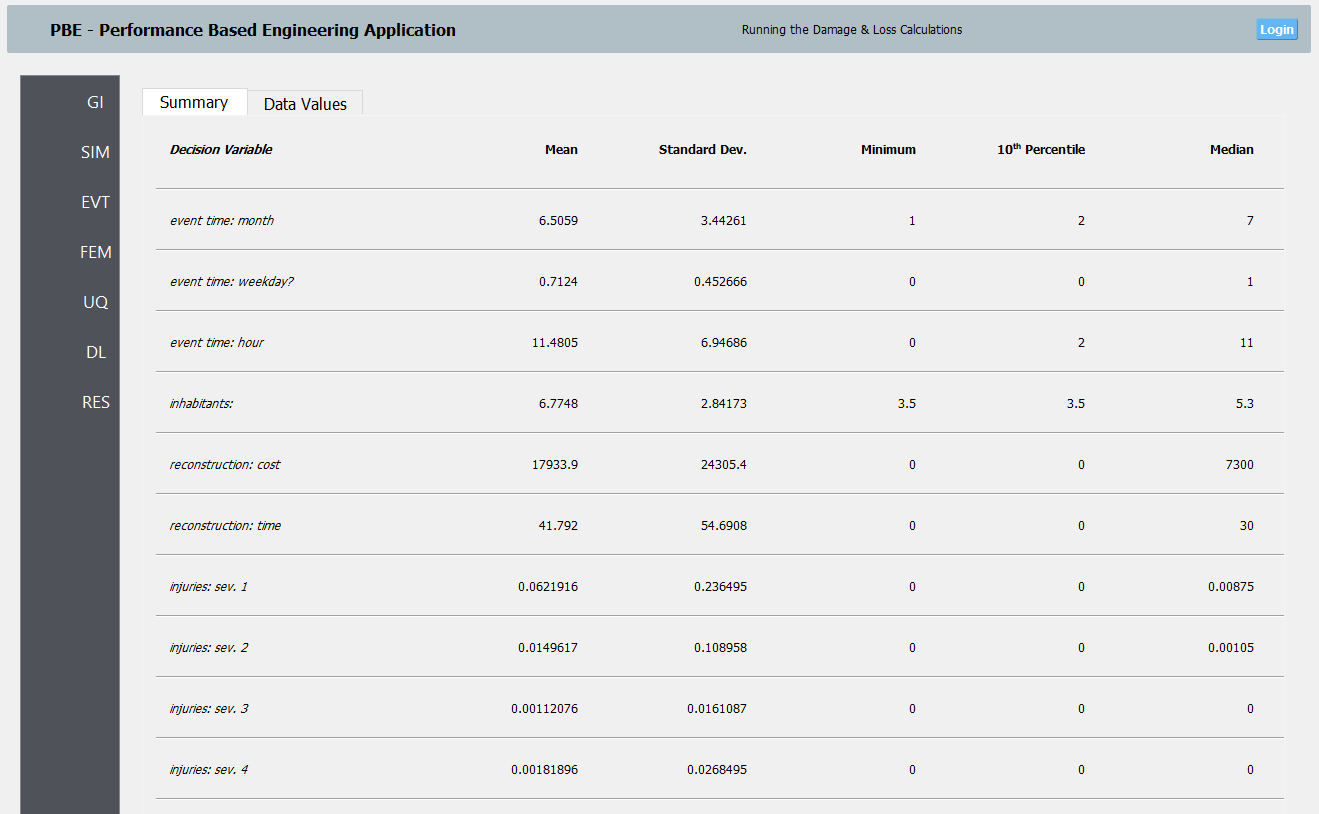
\includegraphics[width=0.95\textwidth]
    {installation/figures/test_uq_res_pbe.png} }
  \caption{Results for test analysis. This tab will open automatically
  when the analysis completes, indicating a successful installation}
  \label{fig:show_results}
\end{figure}
}{
\begin{figure}[!htbp]
  \centering {
    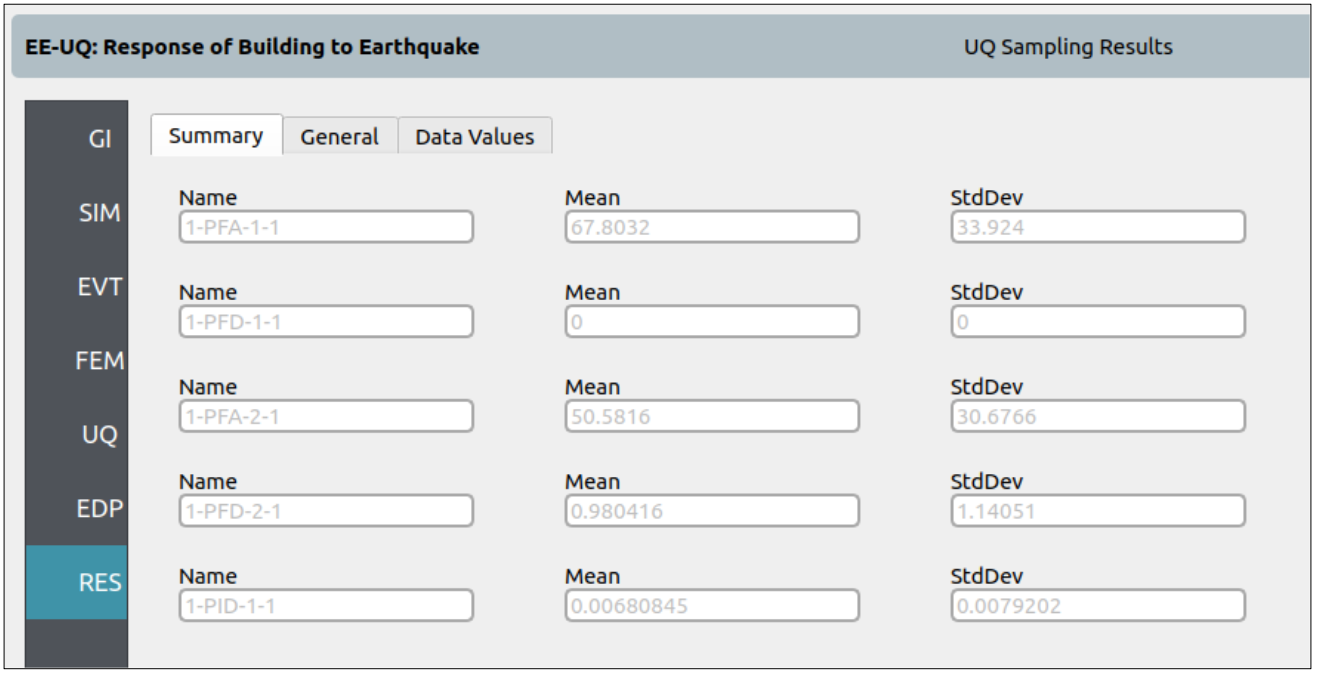
\includegraphics[width=0.7\textwidth]
    {installation/figures/test_uq_res.png} }
  \caption{Results for test analysis. This tab will open automatically
  when the analysis completes, indicating a successful installation}
  \label{fig:show_results}
\end{figure}
}

If successful, the application will pause briefly while it runs the
analysis before automatically displaying the simulations results in
the \texttt{RES} tab, as shown
in \Cref{fig:show_results}. Remember, the results shown
in \Cref{fig:show_results} most likely will not be the same as
those from this local test since $V_{S_{30}}$ is a random variable and
the values realized in the simulations will be different while still
following the same distribution. In any case, if the simulations
completed and the \texttt{RES} tab is showing simulation results, then
the \texttt{\getsoftwarename{}} App is properly installed and configured.
